\documentclass{article}

% NeurIPS 2026. Submission build takes no option: the style file anonymises the paper and
% adds line numbers, as the call for papers requires. --preprint passes [preprint] for the
% arXiv copy. [final] is only for accepted papers and is never emitted here.
\usepackage[preprint]{neurips_2026}

\usepackage[utf8]{inputenc}
\usepackage[T1]{fontenc}
\usepackage{url}
\usepackage{booktabs}
\usepackage{amsfonts}
\usepackage{amsmath}
\usepackage{nicefrac}
\usepackage{microtype}
\usepackage{graphicx}
\usepackage{xcolor}
\usepackage{hyperref}

\title{Attention-Sink Signatures Dissociate During Vision--Language Pretraining}

\author{  Samvat Tiwari \\
  Independent Researcher \\
  \texttt{samvat.t@gmail.com} \\
}

\begin{document}

\maketitle


\begin{abstract}
Attention sinks, token positions that draw heavy attention while contributing little, are a widely studied target of interventions in language models and are often linked, though not causally, to hallucinations in vision-language models. A sink is defined by attention concentration ($\mathrm{Sink}^{\epsilon}_{1}$), but in text LMs it reliably arrives with two companions: a drained value norm (v-ratio) and massive activations (h-ratio) at the same position. We measure these three signatures during multimodal pretraining: a 222M vision-language model with a randomly initialized decoder, position 0 being an image token, no BOS, trained under four levers: softmax attention, output-gated softmax, unnormalized sigmoid attention, and initialization from a pretrained text LM. We find that the signatures come apart, across 2-3 seeds, depending on which train-time lever was applied. Most notably: on a 1B fresh-token run (2.39 effective visual epochs, single seed), the massive-activation proxy more than doubles while attention concentration stays at exactly zero at every threshold we test. Value-norm drain emerges as a third axis, apart from the massive-activation vs. sink dissociations known from text-only models.
\end{abstract}


\section{Introduction}

Decoder-only transformers pick up a habit early in training: a large share of attention goes to the first token or tokens of a sequence, whatever they contain. The habit carries practical weight --- streaming inference depends on it \cite{ref1}, the extreme activation outliers that ride along with it make quantization harder \cite{ref2}, and a survey now organizes a subfield around interpreting and removing it \cite{ref3}.

The sink does not arrive alone. In text language models three measurements move together: attention concentrates on the sink token, the value vector there drops to a near-zero norm, called value-state drain \cite{ref4}, and the residual stream there grows an abnormally large norm, called a massive activation \cite{ref2,ref5}. These effects settle on the same few tokens \cite{ref6} and appear near step 1000 \cite{ref7}, and the field has taken the co-occurrence as licence to treat all three as facets of one attention-sink phenomenon.

Whether they really are one phenomenon is contested. One line argues for causal unity: massive activations mathematically require representational compression, and ablating them removes both compression valleys and sink formation \cite{ref7}. A related view holds that outlier-driven rescaling by attention and residual sinks is \textit{essential} to stable training \cite{ref8}. Two recent studies pull the other way, each separating a pair of the signatures by intervention --- normalization scheme \cite{ref9}, value scale \cite{ref10}. Both are text-only, and each separates at most two of the three.

Which signature a study measures therefore decides what it can conclude. If the three move independently, a lever that clears concentration while leaving the value path alone reads as a fix under one metric and a failure under the next, and two papers can disagree while both are right. The stakes reach past bookkeeping: sink-like attention has been tied to hallucination and weak visual grounding in deployed vision--language models \cite{ref13,ref14,ref15,ref16}. We measure all three at once, throughout training, and test no downstream behavior.

Vision--language models make a sharp instrument for the question, because the multimodal setting changes what position 0 \textit{is}: our sequence starts with 49 image tokens and has no BOS token, so the candidate sink token is a visual token, without the special-token machinery that text-LM sink accounts lean on. The multimodal sink studies we know analyze mostly frozen, already-trained backbones at inference time \cite{ref11,ref12}, and the one training-time view follows a single magnitude rather than three signatures (\S4). Whether the signatures arrive together, in sequence, or independently takes a randomly initialized decoder with all three logged separately from step 0.

We work at deliberately small scale: a 222M-parameter nanoVLM \cite{ref17}, where a pretrained SigLIP-B/16 encoder \cite{ref18} feeds a randomly initialized decoder with the SmolLM2-135M architecture \cite{ref19}. Four levers each target one sink-relevant mechanism (\S2): standard softmax attention (\textit{baseline}), a Qiu-style G1 output gate in our zero-initialized variant \cite{ref20} (\textit{g1gate}), unnormalized sigmoid attention, which removes the normalization sinks are argued to come from \cite{ref6} (\textit{sigmoid}), and initialization from the pretrained SmolLM2 text model (\textit{textinit}). A validated probe logs all three signatures every 100 steps. The four-arm comparison reuses a small image pool, so we re-test the central negative result under low repetition, on a fresh stream of one billion tokens (\textit{RF}, 2.39 effective visual epochs).

\textbf{Contributions.}

\begin{enumerate}
  \item \textbf{Four levers, four corners (n = 2--3 seeds/arm).} The arms reach four different corners of the three-signature space, no two sharing a triple. The value-norm ratio alone is strongly drained, mildly drained, or amplified, depending on the lever (Fig. 1, Table 1). The arms are not a factorial design, so we report intervention-associated profiles, not isolated causal effects.
  \item \textbf{Low-repetition decoupling at 1B tokens (n = 1).} On a fresh stream at 2.39 effective visual epochs, with training healthy throughout (\S2), the massive-activation proxy rises from an h-ratio of 1.43 to 3.22, about 2.3$\times$, while concentration stays at exactly zero and no head ever crosses the sink threshold (\S3.2, \S5).
  \item \textbf{No consistent-sign head-level relationship.} The per-head correlation between concentration and value-norm flips sign across arms at seed 0 (+0.76 baseline $\rightarrow$ $-$0.79 textinit, pooled $-$0.20, over 90 KV groups per arm), reported descriptively (\S3.3).
\end{enumerate}

Decoupling itself is not new \cite{ref9,ref10} and we do not claim it. The new part is the conjunction --- all three signatures tracked jointly under randomly initialized decoders in a multimodal model, with value-norm drain as a third axis.

\section{Setup}

\paragraph{Model and token layout} All runs use a 222M-parameter nanoVLM \cite{ref17}: a pretrained, trainable SigLIP-B/16 vision encoder \cite{ref18} feeding a decoder with the SmolLM2-135M architecture \cite{ref19} through a learned modality projector. The decoder has 30 layers of grouped-query attention, 9 query heads per layer sharing 3 KV heads: 270 (layer, query-head) pairs but only 90 (layer, KV-group) value projections, a distinction that matters in \S3.3. It trains \textbf{from random initialization} in every arm except \textit{textinit}, the designed exception, importing first-position structure from text pretraining (\S3.1). Each sequence holds 49 image tokens as a causal prefix, then 79 left-padded text tokens, 128 in all. \textbf{Position 0 is the first image token, and there is no BOS token} (\S1).

\paragraph{Arms} Four training levers, each targeting one sink-relevant mechanism. Everything else stays byte-identical across arms.

\begin{table}[t]
  \centering
  \begin{tabular}{lllcl}
    \toprule
    arm & attention & LM init & ViT init & lever precedent \\
    \midrule
    \textit{baseline} & softmax & random & pretrained & --- \\
    \textit{g1gate} & softmax + elementwise $\sigma$-gate (zero-init, post-SDPA) & random & pretrained & G1 gating \cite{ref20} \\
    \textit{sigmoid} & unnormalized sigmoid, no softmax & random & pretrained & Gu et al. \cite{ref6} \\
    \textit{textinit} & softmax & pretrained SmolLM2-135M & pretrained & --- (novel control) \\
    \bottomrule
  \end{tabular}
\end{table}

The \textit{g1gate} and \textit{sigmoid} levers have established sink effects in text-only models \cite{ref20,ref6}. \textit{textinit} has no precedent there: an inheritance control, carrying in whatever sink structure text pretraining built into SmolLM2.

\paragraph{A scale confound in our gate variant} Unlike Qiu et al. \cite{ref20}, we initialize the G1 gate at exactly zero, so it opens at $\sigma$(0) = 0.5 and the arm begins as a half-scale output intervention as well as a gating one --- \textbf{Qiu-style G1 in our zero-initialized variant} throughout (\S5).

\paragraph{Data and the two training regimes} The four-arm comparison trains on four curated subsets of \texttt{the\_cauldron} \cite{ref21}, about 146K images, matched at about 100M tokens per arm. \textit{textinit} stops at 60M, where its signatures have plateaued (\S3.1). Reuse of that pool gives high visual-epoch counts, the objection the \textbf{RF} arm (random-fresh) answers (\S3.2): the \textit{baseline} recipe re-trained on a fresh FineVision stream \cite{ref22} to 1B tokens, over about 4.6M natural images, at \textbf{2.39 effective visual epochs} --- a \textbf{low-repetition} run, not a repetition-free one, since examples repeat about 2.4 times on average. We estimate the overlap between the fresh pool and the repeated subsets at under 3\%, from config-level composition rather than image-level deduplication. Swapping datasets trades the repetition confound for a domain-shift confound, which \S5 takes up.

\paragraph{Three signatures, tracked separately} We log the three sink symptoms the text-LM literature reports together, each at its own granularity, following Gu et al. \cite{ref6} at fixed sequence length. The decoder has \textit{L} = 30 layers, \textit{H} = 9 query heads and \textit{G} = 3 KV heads per layer. Every quantity below is averaged over valid query positions and over the fixed probe batch.

\textit{Concentration} ($\mathrm{Sink}^{\epsilon}_{1}$) is the fraction of the \textit{L$\cdot$H} = 270 (layer, query-head) pairs whose mean attention to position 0 exceeds $\epsilon$. We use the $\epsilon$ = 0.3 default of \cite{ref6} and check $\epsilon$ $\in$ \{0.2, 0.4\}. Cross-arm tables report the stricter $\epsilon$ = 0.2, which makes an absence claim harder to pass.

\textit{Value-norm ratio} (v-ratio) is the value norm at position 0 divided by the mean value norm over the other valid positions, per layer and averaged over the 30 layers. Below 1 is value-drain \cite{ref4}, above 1 amplification. Under grouped-query attention a value vector belongs to a KV group and repeats across 3 query heads, so the ratio rests on \textit{L$\cdot$G} = 90 distinct value projections, not 270 (\S3.3).

\textit{Residual-norm ratio} (h-ratio) is the residual-stream norm at position 0 divided by the mean norm over the other positions, again per layer and averaged over the 30 layers. We call it a \textbf{massive-activation proxy}, because massive activations are normally defined by channel-level outliers \cite{ref2,ref5}, which we never measured (\S5).

All three metrics \textbf{anchor on position 0 by construction}, a measurement choice we check: at seed 0, per-position attention mass makes position 0 the maximum-mass token in every arm (Appendix C), and \S5 handles the remaining seed-level caveat. The \textit{sigmoid} arm reports the row-normalized attention view, which keeps concentration comparable across arms, and we also log the raw sigmoid mass (Appendix D).

\paragraph{Why a sink is expected at all} Softmax forces every attention row to sum to one, so a head with nothing worth retrieving must still put its mass somewhere \cite{ref6}. Our \textit{sigmoid} arm removes that constraint and tests it directly.

\paragraph{Probe} The function \texttt{probe\_sinks()} re-walks the decoder from the live module weights in eager mode, fp32, no gradients, independent of the training path (fused SDPA kernels, autocast, \texttt{torch.compile}). Every call validates its hidden states against the real forward pass to a relative error below 10$^{-2}$, so the probe cannot drift from what the trained model computes. The probe batch is fixed across all runs and seeds, keeping every number comparable, and probes fire every 100 optimizer steps, dense enough to timestamp each signature's first threshold crossing. Appendix F gives the probe batch, token accounting and validation protocol.

\paragraph{Recipe} AdamW with weight decay 0.1, following \cite{ref6}, gradient clip 1.0, cosine schedule with 3\% warmup. Arms in a comparison differ only in the lever under test. Two seeds for \textit{baseline} and \textit{sigmoid}, three for \textit{g1gate} and \textit{textinit}, one for \textit{RF}. Appendix F gives the learning rates, precision and batch size.

\paragraph{Validation losses, and what they license} Training stays healthy in all reported runs. At the matched 100M-token checkpoint the held-out losses are 1.182 for \textit{baseline}, 1.133 for \textit{g1gate}, 1.206 for \textit{sigmoid} and 0.877 for \textit{textinit}, and RF reaches 0.638 at 1B tokens (Appendix F). Two cautions. \textit{textinit} starts from a pretrained text decoder, so its lower loss reflects unequal competence, not a lever effect: only \textit{baseline}, \textit{g1gate} and \textit{sigmoid} are equal-token, equal-initialization comparisons. And the repeated-data arms show a large train--validation asymmetry (\texttt{val\_seen} near 0.44 against \texttt{val\_unseen} near 1.18), the overfitting signal that motivates RF. RF has no seen split, so the weaker statement its data supports is a held-out loss with a negative fitted slope over the second half, ending at 0.638, with individual evaluations fluctuating (\S5). \textbf{We did not run MMStar or any other downstream benchmark on any arm}, so this paper makes no capability claim (\S5).

\section{Results}

\begin{figure}[t]
  \centering
  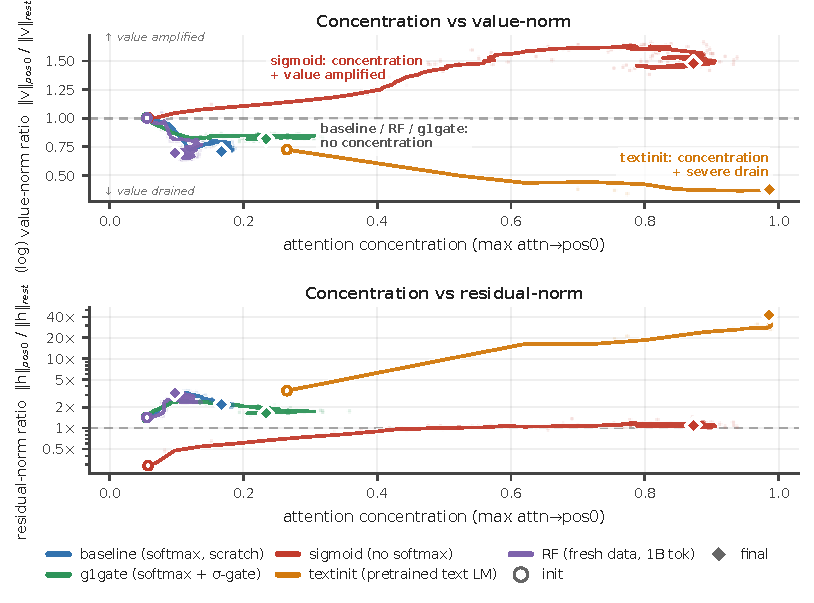
\includegraphics[width=0.8\linewidth]{figures/fig2_phase_portrait.pdf}
  \caption{\textbf{Figure 1: Decoupling phase-portrait.} Every arm in concentration-against-value-norm space (left) and against the residual-norm ratio (right, log scale). Circles mark initialization, diamonds the final checkpoint (about 100M tokens, 60M for \textit{textinit}, 1B for \textit{RF}). Seed 0 unless labelled. \textbf{The horizontal axis is the \textit{maximum} attention$\rightarrow$pos0 over heads, not Table 1's fraction above threshold}, so an arm can sit off zero here with Sink$^{\epsilon}$ = 0.000. Paths smoothed, end markers raw (Appendix D). Were the three signatures one phenomenon, these trajectories would move along one direction.}
  \label{fig:fig1}
\end{figure}

\subsection{Four training levers reach four different signature corners}

Table 1 collapses the seeds into per-arm ranges, each arm at its final matched checkpoint: about 100M tokens, 60M for \textit{textinit}, whose signatures have plateaued by then (per-seed table in Appendix B). \textbf{No two arms share a signature triple.}

\begin{table}[t]
  \centering
  \caption{Table 1 --- the four corners (n = 2--3 seeds per arm).** Concentration is $\mathrm{Sink}^{0.2}_{1}$, the fraction of the 270 (layer, query-head) pairs whose mean attention$\rightarrow$pos0 exceeds 0.2. The v-ratio rests on 90 (layer, KV-head) value projections and the h-ratio on 30 layers (\S2).}
  \begin{tabular}{llll}
    \toprule
    arm & concentration & value-norm & massive-activation proxy \\
    \midrule
    baseline & absent (0.000) & mild drain (0.69--0.72) & moderate (1.7--2.2) \\
    g1gate & near-absent (0.004--0.011) & \textbf{milder drain} (0.81--0.85) & moderate (1.7--2.2) \\
    sigmoid & strong (0.76--0.83) & \textbf{amplified} (1.48--1.60) & no strong asymmetry (1.1--1.3) \\
    textinit & strong (0.56--0.85) & strong drain (0.38--0.63) & extreme (5.5--42.5) \\
    \bottomrule
  \end{tabular}
\end{table}

The value-norm axis alone takes three directions --- drained hard, drained mildly, amplified --- and the corners separate pairwise on single axes. \textit{g1gate} differs from \textit{baseline} on the value-norm axis alone: concentration absent or near-absent and the residual-norm ratio moderate in both, while the gate makes the baseline's mild drain milder still, a 15--19\% drain rather than none. \textit{sigmoid} and \textit{textinit} both reach strong concentration and then part on the \textit{direction} of the value-norm move and on the residual-norm ratio. The \textit{sigmoid} corner is relative: its concentration is row-normalized over a shrinking raw gate budget, with top-head raw pos0 mass 0.065 at the final checkpoint (Appendix D). The arms are not a factorial design, so we report distinct intervention-associated profiles rather than isolated causal effects of single levers. The trajectories in Figure 1 separate early and do not share one origin: \textit{textinit} starts from a pretrained text decoder that already carries a subthreshold first-position bias, with $\mathrm{Sink}^{0.3}_{1}$ still 0.000 at step 0.

Reproducibility differs by arm. \textit{g1gate} is tightest, $\mathrm{Sink}^{0.2}_{1}$ of 0.004, 0.011 and 0.0037 across three seeds. The corner of \textit{textinit} repeats across seeds and its magnitudes do not: seed 0 sits far above the other two on every signature at once, h-ratio 42.5 against 5.5--12.2, partly because at seeds 1 and 2 its peak signatures move off position 0, where our metrics anchor (Appendix B, H). We therefore report textinit's massive-activation proxy as a \textbf{range (5.5--42.5$\times$) with a median near 12$\times$} throughout, and treat the corner as the reproducible claim rather than any magnitude.

\paragraph{The corners also separate in time} (Appendix H, Fig. A4, seed 0). The random-decoder softmax arms, \textit{baseline}, \textit{g1gate} and \textit{RF}, cross the norm thresholds without ever crossing concentration. \textit{sigmoid} is the mirror image, crossing concentration without either norm threshold. \textit{textinit} starts above both norm thresholds and crosses concentration later. Where a run crosses both kinds, the norm signatures come first, and under text initialization the three need not even settle on the same token (timings, positional scan and entropy-collapse correlate in Appendix H, Appendix E sets out, as untested hypotheses, how each lever might move a different axis).

Figure 2 shows the separation inside a single head. Its rightmost panel carries the most weight: \textbf{the textinit stripe is already there at step 0}, imported with the text-LM weights before the model has seen one image.

\begin{figure}[t]
  \centering
  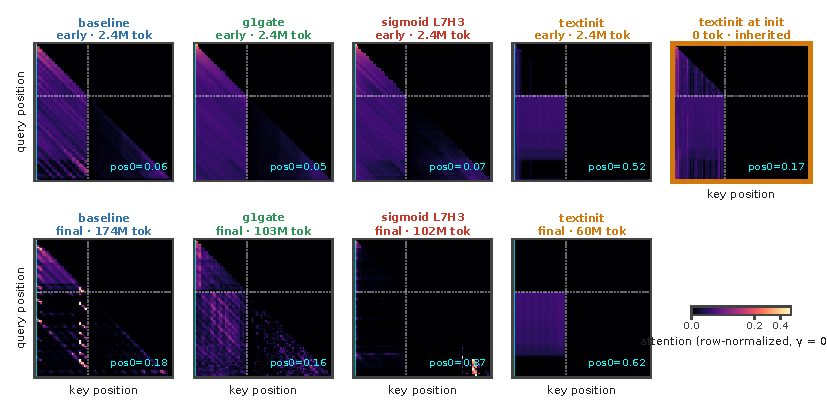
\includegraphics[width=0.8\linewidth]{figures/fig6_sink_stripe.pdf}
  \caption{\textbf{Figure 2: The sink stripe.} Query \&times; key attention of each arm's top sink head, row-normalized, seed 0. Top row is early training (step 250, about 2.4M tokens), bottom row the final checkpoint. The cyan line marks key = pos0, the dotted line the image-to-text boundary. The stripe is \textit{absent} in baseline throughout, strong in textinit (attn$\rightarrow$pos0 = 0.62 at its final checkpoint), and \textit{already present at step 0} in textinit (rightmost panel), inherited from the text LM. The sigmoid column's heat maps come from an auxiliary streaming batch, while every printed sigmoid number comes from the fixed probe batch (Appendix D).}
  \label{fig:fig2}
\end{figure}

\subsection{The proxy grows across 1B low-repetition tokens with concentration at zero}

The four-arm comparison reuses a 146K-image pool, so a reader could read its ``concentration never emerges'' result as an overfitting artifact. The RF arm answers that: the identical \textit{baseline} recipe on a fresh FineVision stream to one billion tokens at \textbf{2.39 effective visual epochs}, a \textbf{low-repetition} run rather than a repetition-free one. Its held-out loss has a negative fitted slope over the second half of training and ends at 0.638, while individual evaluations fluctuate (\S2, \S5).

Concentration never arrives: \textbf{$\mathrm{Sink}^{0.3}_{1}$ = 0.000 across the entire 0 $\rightarrow$ 1B run}, no head of the 270 crossing the threshold at any of about 700 probes. The massive-activation proxy meanwhile keeps growing far past warmup.

\begin{table}[t]
  \centering
  \caption{Table 2 --- RF (fresh stream, n = 1 seed), init $\rightarrow$ 1B tokens.}
  \begin{tabular}{lccl}
    \toprule
    signature & @ init & @ 1B & net \\
    \midrule
    $\mathrm{Sink}^{0.3}_{1}$ (concentration) & 0.000 & 0.000 & flat zero, entire run \\
    max attn$\rightarrow$pos0 & 0.056 & 0.098 & $\approx$flat, far below threshold \\
    h-ratio (massive-activation proxy) & 1.43 & \textbf{3.22} & \textbf{$\approx$2.3$\times$}, positive long-horizon trend \\
    v-ratio (value-norm) & 1.00 & 0.69 & net drain, non-monotone \\
    \bottomrule
  \end{tabular}
\end{table}

Warmup does not explain the rise: the h-ratio climbs from 2.40 at about 57M tokens to 3.22 at 1B, long after the 3\% warmup window closes, though not monotonically at probe resolution, hence a positive long-horizon trend. In Figure 1, right, the violet trajectory climbs and never moves rightward. The v-ratio ends below its initialization value, but about 75\% of that drop happens in the first 57M tokens and part then recovers, so we report it as supporting context rather than ongoing emergence.

\subsection{No consistent-sign head-level concentration--value-norm relationship}

A tight coupling between concentration and value-drain should at minimum hold the sign of their per-head correlation constant across regimes. It does not. Table 3 gives the Pearson r between attention$\rightarrow$pos0 and value-norm ratio at each arm's final checkpoint, seed 0, over the 90 (layer, KV-group) observations, averaging a group's query-head attention rather than triplicating its value observation (\S2, scatter in Fig. A2).

\begin{table}[t]
  \centering
  \caption{Table 3 --- r(attn$\rightarrow$pos0, v-ratio), final checkpoint, seed 0.}
  \begin{tabular}{lccccc}
    \toprule
    baseline & g1gate & sigmoid & textinit & RF & pooled \\
    \midrule
    +0.76 & +0.57 & $-$0.03 & $-$0.79 & +0.51 & $-$0.20 \\
    \bottomrule
  \end{tabular}
\end{table}

These correlations are \textbf{descriptive, not inferential}: heads within a layer are not independent and each arm rests on a single seed here, so a p-value would mislead and we report none. Collapsing to the 90 KV groups removes the pseudoreplication a per-query-head reading would introduce, leaving the picture unchanged (Appendix D).

The pattern is about \textbf{sign}, which pseudoreplication does not manufacture: heads attending more to position 0 have \textit{larger} value norms in the baseline regime and \textit{smaller} ones under text initialization, and the pooled correlation is weak only because arms of opposite sign cancel. We claim no consistent-sign relationship across arms --- not the absence of a coupling law, though a fixed coupling would show one sign everywhere, and it does not.

\section{Related work}

\paragraph{Attention sinks and their companions in text language models} Gu et al. \cite{ref6} give the canonical account: the sink token acts ``more like key biases, storing extra attention scores,'' carries small key and value norms as part of the same phenomenon, and connects to massive residual-stream activations \cite{ref2,ref5}. They also show unnormalized sigmoid attention prevents sink formation in text models up to 1B parameters, which our \textit{sigmoid} arm builds on. Guo et al. \cite{ref4} call the concentration and value-drain coupling ``active-dormant'' heads. Queipo-de-Llano, Arroyo et al. \cite{ref7} make the strongest unity claim and the only genuinely \textit{causal} one: massive activations mathematically require representational compression, and ablating a model's layer-0 massive activation removes both compression valleys and sink formation. We reserve ``causally unified'' for that result alone. Peng et al. \cite{ref24} trace a first-position sink circuit emerging early in from-scratch text pretraining, without separating the signatures.

\paragraph{Prior decoupling results: text-only, two axes} Two papers already separate pairs of these signatures, and we scope our claim around them. Sun, Canziani, LeCun and Zhu \cite{ref9} show massive activations and attention sinks are dissociable architectural artifacts: a change of normalization scheme crushes the massive-activation spike while the sink ratio survives. Chen and Yao \cite{ref10} decouple the same pair from the opposite direction and from scratch: a value-scale intervention in 0.1--0.3B text models keeps the sinks and suppresses massive activations. Neither treats value-norm drain as a third axis, and neither is multimodal. Fesser et al. \cite{ref23} give the closest external support for tracking the value norm separately: one sink pattern can hide an ``adaptive nop'' (negligible value norms) or a ``broadcast'' that redistributes global information (low-rank outputs), though that work diagnoses trained vision transformers rather than tracking emergence. Qiu et al. \cite{ref8} argue the opposite case, that outlier-driven rescaling by attention and residual sinks is essential to stable training. The field has settled neither question.

\paragraph{Multimodal sinks: mostly frozen backbones, inference time} Luo et al. \cite{ref11} separate ViT-propagated from LLM-emerged sinks. Their Appendix A.4 tracks sink-dimension magnitudes across alignment checkpoints, so a training-time view has precedent, though on a frozen vision transformer with a pretrained language model, following one magnitude rather than three signatures. Choi et al. \cite{ref12} likewise distinguish vision-sinks from language-sinks in a frozen model and gate them by layer. Both establish distinct vision-side and language-side origins, which our \textit{textinit} inheritance result fits. What is missing is dense, joint tracking of the three quantities in a decoder that starts from random weights. Vision transformers also grow high-norm ``register'' tokens of their own \cite{ref25}, hence the pretrained-encoder limitation in \S5. A separate line ties these signatures to hallucination and grounding failure in deployed models and intervenes at inference time \cite{ref13,ref14,ref15,ref16}, the practical reason it matters which signature a mitigation moves.

\paragraph{The gating lever} Qiu et al. \cite{ref20} introduce the head-specific elementwise sigmoid gate on attention output that our \textit{g1gate} arm adapts. In text models it ``largely reduces the attention score allocated to the first token and decreases massive activations'' while improving quality. Our zero-initialized variant confounds gating with initial output scaling (\S2, \S5). With that caveat, concentration is already absent in our baseline, so the gated arm differs on the value-norm axis: the drain becomes milder, 0.69--0.72 to 0.81--0.85, rather than disappearing --- invisible unless the three signatures are logged separately.

\paragraph{Positioning} The closest prior work separates at most two of the three axes, in text-only models, and the multimodal studies work mostly on frozen ones. Our claim is the conjunction: \textbf{concentration, value-norm drain and the residual-norm ratio tracked jointly and separately in multimodal pretraining with a randomly initialized decoder}, adding value-norm drain as a third axis beyond the text-only dissociations \cite{ref9,ref10}. Decoupling itself is not ours, and prior multimodal work could study emergence if it chose to.

\section{Limitations}

\paragraph{Metrics anchored on position 0} We measure all three signatures at the first image token, checked by per-position attention \textit{mass} rather than argmax alone: position 0 is the maximum-mass token in every arm at seed 0, and stays so for \textit{baseline}, \textit{g1gate} and \textit{sigmoid} at every seed we scanned. It does \textbf{not} in \textit{textinit}, where at seeds 1 and 2 the peaks move to other positions (per-position table in Appendix C). The pos0-anchored textinit magnitudes at those seeds therefore \textit{understate} its peaks, one more reason to treat that arm's corner rather than its magnitudes as the claim. In \textit{RF} the attention argmax sits at pos1, but with mass 0.053 against 0.044 at pos0, a diffuse profile rather than a displaced sink, so the RF result does not depend on the anchor.

\paragraph{The gate arm carries a scale confound} We initialize the G1 gate at exactly zero, so it opens at $\sigma$(0) = 0.5 and halves attention output at step 0, where Qiu et al. \cite{ref20} use ordinary initialization (\S2). Gating and initial output scaling are therefore confounded in \textit{g1gate}: its differences from baseline cannot be attributed to gating alone, and a scale-matched control is future work.

\paragraph{Pretrained vision encoder: no arm is fully from scratch} The SigLIP encoder is pretrained and trainable in every arm, and \textit{textinit} also uses a pretrained decoder. We study vision--language pretraining with randomly initialized decoders, not from-scratch training of the whole model. Vision transformers grow high-norm register tokens of their own \cite{ref25}, and sinks can propagate from a vision transformer into a vision--language model \cite{ref11}, so part of our residual-norm signal could be inherited rather than decoder-formed. Our defense is the trajectory: the h-ratio starts at 1.0--1.4 and \textit{rises} to 3.22 across 1B tokens in RF, where inheritance from a static encoder predicts a high, flat h-ratio from step 0. A randomly initialized vision transformer, which would isolate the decoder, is future work.

\paragraph{The h-ratio is a proxy, not a measurement of massive activations} Massive activations are normally defined by channel-level outliers \cite{ref2,ref5}. We measured a position-specific residual-norm ratio and never computed channel-level statistics (\S2). A large h-ratio is consistent with massive activations without establishing them.

\paragraph{Token scale} Our runs reach at most 1B tokens per arm, against the roughly 5B canonical in the text-LM sink literature \cite{ref6}. Text-LM sinks form near step 1000 \cite{ref7}, far inside our range, but a signature absent at 1B could still emerge later.

\paragraph{Reproducibility of textinit magnitudes} The massive-activation proxy of \textit{textinit} is seed-sensitive, an h-ratio of 5.5--42.5 across three seeds, with seed 0 the outlier on every signature. The corner --- strong concentration, strong drain, large residual-norm ratio --- is the reproducible claim. No specific magnitude is.

\paragraph{Provenance and seed count} The seed-0 raw probes for the four-arm comparison come from a checksummed archive summary rather than first-hand re-derivation. Seeds 1 and 2 we \textit{did} re-derive independently, an audit that caught a metric-labeling error in an earlier internal consolidation (Appendix G). \textit{baseline} and \textit{sigmoid} have two seeds, \textit{g1gate} and \textit{textinit} three, RF a \textbf{single seed}. RF also contains one \textbf{weights-only optimizer restart at about 57M tokens}, forced by an out-of-memory error: weights reloaded, AdamW moment estimates discarded, so RF is not one uninterrupted optimizer trajectory. The audit verified continuity across that seam: v-ratio and h-ratio identical at the shared checkpoint, a double-covered 600-step overlap diverging only within probe noise, concentration 0.000 on both sides. Concentration was reproducibly zero across both repeated-data baseline seeds, adequate support for the negative claim, and a second fresh-data seed would strengthen it.

\paragraph{What the RF control does and does not establish} RF has no distinct seen split, so we cannot run for it the \texttt{val\_seen} / \texttt{val\_unseen} comparison that exposes memorization in the repeated arms. The weaker statement its data supports is the falling-slope statement of \S2. Its streaming shuffle buffer dropped from 1500 to 500 examples partway through, again for memory, so stream ordering is not homogeneous, though the $\mathrm{Sink}^{0.3}_{1}$ = 0.000 result and the h-ratio rise hold within each regime separately. Its probe batch is still the \textbf{fixed repeated-\texttt{the\_cauldron} tail} used by the other arms, which keeps RF's signatures comparable to theirs --- what the negative result needs --- at the cost of measuring them on data from the other distribution. And RF buys lower repetition by changing dataset, so it trades the repetition confound for a domain-shift one, deliberately and with the fresh pool chosen to minimize shift. The under-3\% overlap figure is config-level, not image-level (\S2), and the third, domain-matched control we did not run is the known follow-up.

\paragraph{We report no benchmark accuracy} We measure sink signatures only (\S2): no downstream benchmark evaluation, such as MMStar, on any arm, and no claim about how signature dissociation relates to downstream capability.

\section{Conclusion}

The coupling is lever-dependent. Across four training levers, the three signatures land in four distinct corners: value norms are strongly drained, mildly drained, or amplified, and on a billion fresh tokens the massive-activation proxy more than doubles while concentration stays at zero. This extends two-way dissociations in text-only models \cite{ref9,ref10} to a third, separately measured axis in multimodal pretraining. In text LMs, massive activations can causally produce sinks \cite{ref7}; our results show the coupling can also fail to form.

The practical implication is simple: across our arms, no one signature was a proxy for the others. A model without a concentration sink can still develop a growing residual-norm asymmetry, and an intervention judged on one signature may leave the others unchanged.

\paragraph{Next steps} A randomly initialized vision encoder, to isolate what the decoder contributes to the residual-norm signal. A fresh-data run past 1B tokens. A scale-matched gate control, to separate gating from the half-scale confound of \S2.

\paragraph{Reproducibility} A self-validating probe (\S2) computes all signatures on a fixed probe batch, from logs taken every 100 steps, and the Appendix holds the per-seed tables. We will release the code, the probe, the run configurations, the per-run logs, and the training checkpoints on acceptance. We withhold the links for double-blind review.

\small
\begin{thebibliography}{25}

\bibitem{ref1}
G. Xiao, Y. Tian, B. Chen, S. Han, M. Lewis. \textit{Efficient Streaming Language Models with Attention Sinks.} ICLR 2024. arXiv:2309.17453.

\bibitem{ref2}
M. Sun, X. Chen, J. Z. Kolter, Z. Liu. \textit{Massive Activations in Large Language Models.} COLM 2024. arXiv:2402.17762.

\bibitem{ref3}
Z. Su et al. \textit{Attention Sink in Transformers: A Survey on Utilization, Interpretation, and Mitigation.} arXiv:2604.10098, 2026.

\bibitem{ref4}
T. Guo, D. Pai, Y. Bai, J. Jiao, M. I. Jordan, S. Mei. \textit{Active-Dormant Attention Heads: Mechanistically Demystifying Extreme-Token Phenomena in LLMs.} CPAL 2025. arXiv:2410.13835.

\bibitem{ref5}
N. Cancedda. \textit{Spectral Filters, Dark Signals, and Attention Sinks.} ACL 2024 (pp. 4792--4808). arXiv:2402.09221.

\bibitem{ref6}
X. Gu, T. Pang, C. Du, Q. Liu, F. Zhang, C. Du, Y. Wang, M. Lin. \textit{When Attention Sink Emerges in Language Models: An Empirical View.} ICLR 2025. arXiv:2410.10781.

\bibitem{ref7}
N. Queipo-de-Llano, D. Arroyo, F. Barbero, Y. Dong, M. Bronstein, Y. LeCun, R. Shwartz-Ziv. \textit{Attention Sinks and Compression Valleys in LLMs are Two Sides of the Same Coin.} arXiv:2510.06477, 2025.

\bibitem{ref8}
Z. Qiu et al. \textit{A Unified View of Attention and Residual Sinks: Outlier-Driven Rescaling is Essential for Transformer Training.} arXiv:2601.22966, 2026.

\bibitem{ref9}
M. Sun, A. Canziani, Y. LeCun, C. Zhu. \textit{The Spike, the Sparse and the Sink: Anatomy of Massive Activations and Attention Sinks.} arXiv:2603.05498, 2026.

\bibitem{ref10}
Y. Chen, Z. Yao. \textit{Attention Sinks Induce Gradient Sinks.} arXiv:2603.17771, 2026.

\bibitem{ref11}
Y. Luo et al. \textit{To Sink or Not to Sink: Visual Information Pathways in LVLMs.} arXiv:2510.08510, 2025.

\bibitem{ref12}
J. Choi, J. Kim, S. Kim, S. Hong, J.-H. Park. \textit{When Sinks Help or Hurt: Unified Framework for Attention Sink in Large Vision-Language Models.} ECCV 2026. arXiv:2604.03316.

\bibitem{ref13}
S. Kang, J. Kim, J. Kim, S. J. Hwang. \textit{See What You Are Told: Visual Attention Sink in Large Multimodal Models.} ICLR 2025. arXiv:2503.03321.

\bibitem{ref14}
T. Shukla, Z. Kira. \textit{SAGE: Sink-Aware Grounded Decoding for Multimodal Hallucination Mitigation.} arXiv:2603.27898, 2026.

\bibitem{ref15}
X. Zhang, Y. Zhu, C. Gu, J. Cao, H. Cheng, K. Wu. \textit{What Drives Attention Sinks? A Study of Massive Activations and Rotational Positional Encoding in Large Vision\&ndash;Language Models.} Information Processing \&amp; Management, 63(2A), art. 104431, 2026. DOI 10.1016/j.ipm.2025.104431.

\bibitem{ref16}
J. Binkowski, K. Adamczewski, T. Kajdanowicz. \textit{Attention Sinks as Internal Signals for Hallucination Detection in Large Language Models.} arXiv:2604.10697, 2026.

\bibitem{ref17}
L. Wiedmann, A. Roy Gosthipaty, A. Marafioti. \textit{nanoVLM.} GitHub repository, 2025. https://github.com/huggingface/nanoVLM.

\bibitem{ref18}
X. Zhai, B. Mustafa, A. Kolesnikov, L. Beyer. \textit{Sigmoid Loss for Language Image Pre-Training} (SigLIP). ICCV 2023. arXiv:2303.15343.

\bibitem{ref19}
L. Ben Allal et al. \textit{SmolLM2: When Smol Goes Big --- Data-Centric Training of a Small Language Model.} arXiv:2502.02737, 2025.

\bibitem{ref20}
Z. Qiu et al. \textit{Gated Attention for Large Language Models: Non-linearity, Sparsity, and Attention-Sink-Free.} NeurIPS 2025. arXiv:2505.06708.

\bibitem{ref21}
H. Lauren\c{c}on, L. Tronchon, M. Cord, V. Sanh. \textit{What Matters When Building Vision-Language Models?} (Idefics2 / The Cauldron). NeurIPS 2024. arXiv:2405.02246.

\bibitem{ref22}
L. Wiedmann, O. Zohar, A. Mahla, X. Wang, R. Li, T. Frere, L. von Werra, A. Roy Gosthipaty, A. Marafioti. \textit{FineVision: Open Data Is All You Need.} arXiv:2510.17269, 2025.

\bibitem{ref23}
L. Fesser, M. Jacobs, T. Fel, A. Keller, S. Kakade. \textit{A Unifying View of Attention Sinks: Two Algorithms, Two Solutions.} arXiv:2606.08105, 2026.

\bibitem{ref24}
R. Peng, R. Li, M. Chen, Y. Zhou, Q. Guo, X. Qiu. \textit{How Attention Sinks Emerge in Large Language Models: An Interpretability Perspective.} arXiv:2603.06591, 2026.

\bibitem{ref25}
T. Darcet, M. Oquab, J. Mairal, P. Bojanowski. \textit{Vision Transformers Need Registers.} ICLR 2024. arXiv:2309.16588.

\end{thebibliography}
\normalsize


\newpage
\appendix

\section{Supporting figures}

\begin{figure}[t]
  \centering
  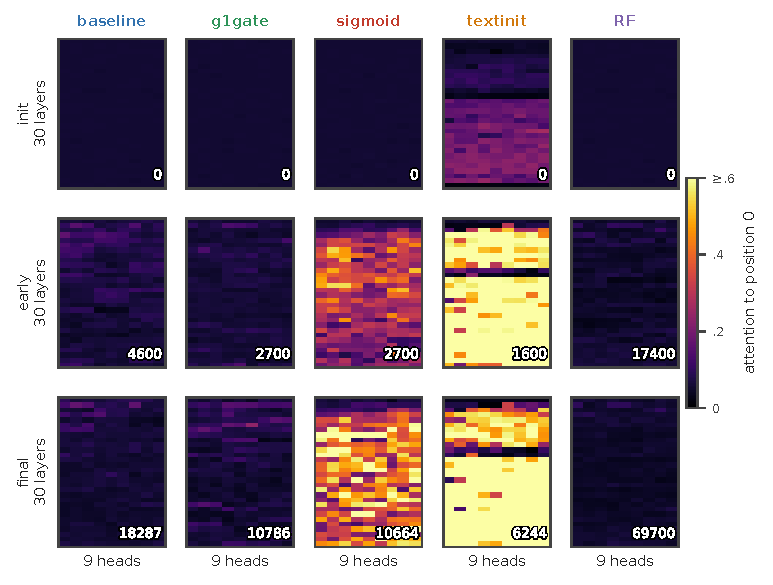
\includegraphics[width=0.8\linewidth]{figures/fig1_layerhead_grid.pdf}
  \caption{\textbf{Figure A1: Where concentration lives in the network.} Mean attention to pos0 for each of the 270 (layer, query-head) pairs through training, row-normalized, seed 0 for every arm, run to each arm's final checkpoint (174M tokens baseline, 103M g1gate, 102M sigmoid, 60M textinit, 1B RF). baseline and RF stay cold throughout. textinit is hot from initialization. sigmoid lights up a band of mid-network layers.}
  \label{fig:figA1}
\end{figure}

\begin{figure}[t]
  \centering
  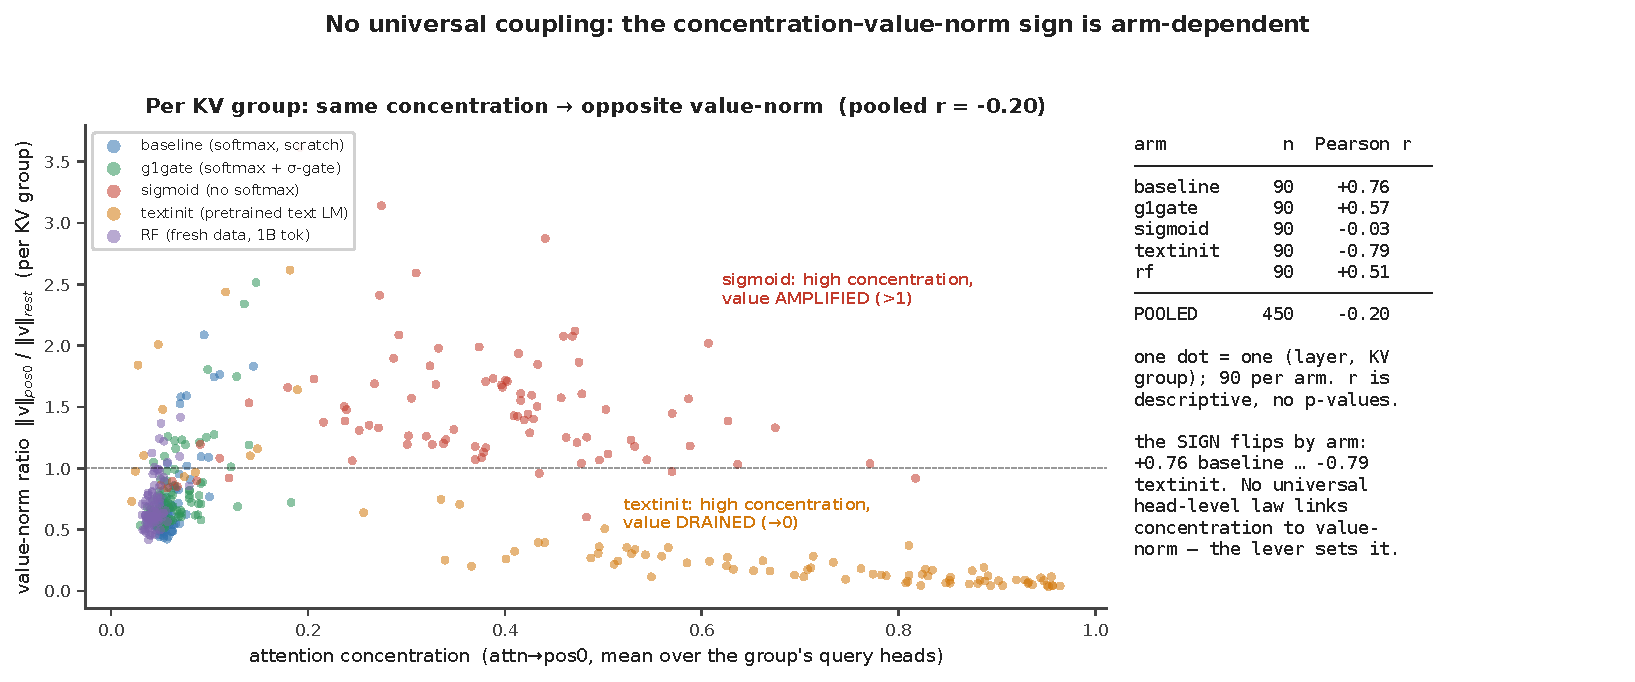
\includegraphics[width=0.8\linewidth]{figures/fig3_perhead_scatter.pdf}
  \caption{\textbf{Figure A2: No consistent-sign head-level relationship.} Concentration against value-norm ratio for each (layer, KV-group) pair at each arm's final checkpoint, seed 0, at n = 90 pairs per arm. Grouping this way avoids triplicating each value-norm observation across the 3 query heads that share it, so these correlations are descriptive and we report no p-values (\&sect;3.3). The sign of the correlation flips by arm, from +0.76 in baseline to \&minus;0.79 in textinit (Table 3). The pooled cloud is weak, at \&minus;0.20, only because arms of opposite sign cancel. Do not read it as an uncorrelated cloud. Most individual arms show a strong |r|.}
  \label{fig:figA2}
\end{figure}

\begin{figure}[t]
  \centering
  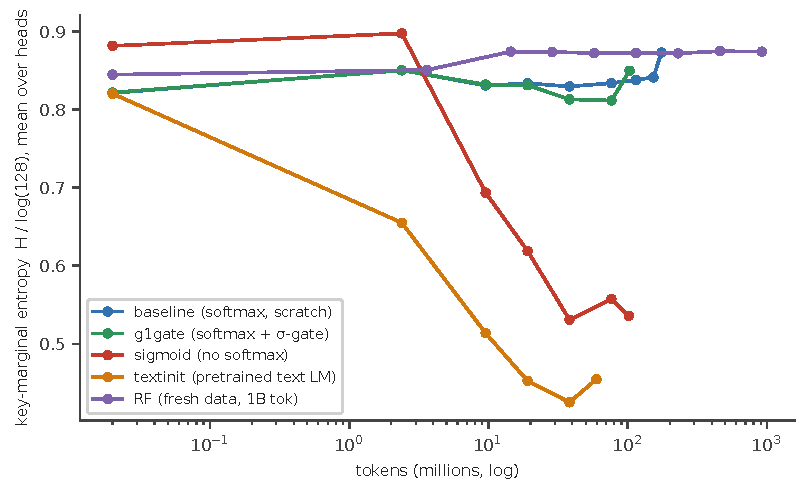
\includegraphics[width=0.8\linewidth]{figures/fig5_entropy.pdf}
  \caption{\textbf{Figure A3: Entropy collapse tracks concentration only.} Mean attention entropy through training, seed 0, to each arm's final checkpoint. Only sigmoid and textinit collapse. baseline, g1gate, and RF stay flat. The entropy-collapse correlate from the text-LM literature therefore follows the concentration axis, not the norm axes.}
  \label{fig:figA3}
\end{figure}

\section{Full per-seed signature table}

This table gives the per-seed values behind the collapsed ranges of Table 1, and adds the maximum attention$\rightarrow$pos0 where we have it. We logged that metric for seeds 1 and 2 only, because the seed-0 archive summary does not include it. We trust the seed-0 values from a checksummed archive rather than re-derive them first-hand (\S5). Each arm is read at its final matched checkpoint. All three signatures of \textit{textinit} have plateaued at 60M tokens, and its h-ratio changes by less than 10\% from 60M to 100M in the seeds that continued.

\begin{table}[t]
  \centering
  \begin{tabular}{lccccccc}
    \toprule
    arm & seed & tokens & $\mathrm{Sink}^{0.2}_{1}$ & mean attn$\rightarrow$pos0 & max attn$\rightarrow$pos0 & v-ratio & h-ratio \\
    \midrule
    baseline & s0 & 101M & 0.000 & 0.068 & --- & 0.723 & 2.16 \\
    baseline & s1 & 100M & 0.000 & 0.062 & --- & 0.687 & 1.71 \\
    g1gate & s0 & 101M & 0.004 & 0.068 & --- & 0.805 & 1.67 \\
    g1gate & s1 & 100M & 0.011 & 0.073 & \textasciitilde{}0.21 & 0.845 & 2.04 \\
    g1gate & s2 & 100M & 0.0037 & 0.072 & \textasciitilde{}0.22 & 0.854 & 2.24 \\
    sigmoid & s0 & 102M & 0.830 & 0.377 & --- & 1.479 & 1.10 \\
    sigmoid & s1 & 100M & 0.756 & 0.311 & --- & 1.603 & 1.30 \\
    textinit & s0 & 60M & 0.852 & 0.627 & --- & 0.377 & 42.5 \\
    textinit & s1 & 60M & 0.556 & 0.235 & \textasciitilde{}0.53 & 0.634 & 5.50 \\
    textinit & s2 & 60M & 0.578 & 0.232 & \textasciitilde{}0.59 & 0.484 & 12.2 \\
    \bottomrule
  \end{tabular}
\end{table}

\textit{baseline} and \textit{sigmoid} are tight across both of their seeds. \textit{textinit} is the loose arm: seed 0 sits far above the other two on every signature at once, at Sink 0.85 against 0.56--0.58, mean attn$\rightarrow$pos0 0.63 against 0.23, and h-ratio 42.5 against 5.5--12.2. The h-ratio has plateaued by 60--100M tokens in both lower seeds, so the spread is genuine seed sensitivity rather than an unconverged transient. Part of it is positional (Appendix C.2).

A note on g1gate. Both seeds with max-attention data show one head at about 0.21--0.22 maximum attention$\rightarrow$pos0. That single head does clear the strict $\epsilon$ = 0.2 threshold, which is why the arm's $\mathrm{Sink}^{0.2}_{1}$ is small but not exactly zero, and no head comes close to the $\epsilon$ = 0.3 default of \cite{ref6}. The arm mean meanwhile stays near 0.07 and $\mathrm{Sink}^{0.2}_{1}$ stays far below 0.05. That pattern repeats across seeds.

\section{Per-position attention mass (seed 0)}

This table gives the mean and max-head attention mass by position at seed 0. It confirms that position 0 is the maximum-mass token in every arm, by mass rather than by argmax count alone. It is the direct check behind the position-0 anchoring defense of \S5.

\begin{table}[t]
  \centering
  \begin{tabular}{lcccl}
    \toprule
    arm & mass@pos0 (mean) & max-head@pos0 & argmax-mass position & reading \\
    \midrule
    baseline & 0.06 & 0.17 & 0 & pos0 max; diffuse (no sink) \\
    g1gate & 0.07 & 0.23 & 0 & pos0 max; diffuse \\
    sigmoid & 0.30 & 0.66 & 0 & pos0 max; broad raw-sigmoid mass \\
    textinit & 0.63 & 0.99 & 0 & pos0 max; razor spike (pos1 = 0.009) \\
    \bottomrule
  \end{tabular}
\end{table}

\subsection{Per-position scan at the remaining seeds, and for RF}

We re-dumped per-position attention mass at the other seeds and for RF, and per-position residual and value norms for all three \textit{textinit} seeds. The table gives the position at which each quantity peaks (for value norms, the position at which the norm is smallest).

\begin{table}[t]
  \centering
  \begin{tabular}{lccccl}
    \toprule
    run & seed & attention-mass argmax & residual-norm peak & value-norm minimum & reading \\
    \midrule
    baseline & s0, s1 & 0 & --- & --- & pos0 max \\
    g1gate & s0, s1, s2 & 0 & --- & --- & pos0 max \\
    sigmoid & s0, s1 & 0 & --- & --- & pos0 max \\
    textinit & s0 & 0 & 0 & 0 & all three coincide \\
    textinit & s1 & 0 & 1 & 5 & norms move off pos0 \\
    textinit & s2 & \textbf{1} & \textbf{13} & \textbf{13} & attention separates from coincident norm extrema \\
    RF & s0 & 1 & --- & --- & mass 0.053 vs 0.044 at pos0, diffuse, not a sink \\
    \bottomrule
  \end{tabular}
\end{table}

Two readings follow. Position 0 remains the maximum-mass token in every arm with a randomly initialized decoder, so the pos0 anchoring holds where the central negative result lives. In \textit{textinit} the three signatures need not share a token, which is the positional dissociation of Appendix H and the reason the pos0-anchored textinit magnitudes at seeds 1 and 2 understate that arm's peaks.

\section{Measurement and rendering details}

\paragraph{Figure 1 smoothing} Paths are smoothed with a moving average, 5 points on the horizontal axis and 9 on the vertical. The faint dots behind each path are the unsmoothed per-probe values, and the initialization and final markers use raw values.

\paragraph{Correlations at the uncollapsed 270 pairs} Table 3 collapses to the 90 (layer, KV-group) observations. At the uncollapsed 270 (layer, query-head) pairs the same quantities read +0.67 for baseline, +0.53 for g1gate, $-$0.03 for sigmoid, $-$0.76 for textinit, and +0.43 for RF. Every sign and every ordering survives the collapse.

\paragraph{Raw against row-normalized sigmoid attention} Row-normalization changes the object being measured, and Gu et al. \cite{ref6} state their result for \textit{unnormalized} sigmoid attention. Head L7H3 of the sigmoid arm sends 0.873 of its row-normalized attention to position 0 at the final checkpoint, which is the arm maximum. Its raw gate mass to position 0 is 0.065, and the raw mass summed over all keys in that row is 0.110. The row does not sum to one, and pos0 takes about 59\% of what little gate mass the head opens at all. Early in training the same head shows the opposite picture: raw pos0 mass 0.309 against a raw row sum of 6.44, so under 5\% of a very large gate budget. The concentration this arm develops is therefore a relative reallocation of a shrinking gate budget onto position 0, not the growth of a large absolute mass there (Appendix H). Raw and row-normalized values here come from the same fixed probe batch as every other number in this paper, masked to valid query positions.

\paragraph{Sigmoid heat-map provenance} The sigmoid column of Figure 2 uses head L7H3 (0-indexed), the arm's top sink head on the fixed probe batch. An earlier dump selected heads by raw, unnormalized gate score, picked different heads, and understated the arm. The sigmoid heat maps are re-rendered from an auxiliary streaming batch, because the saved matrices covered the superseded heads. Every printed sigmoid number, in the text and in the tables, comes from the fixed probe batch. The pos0 share printed on each panel is computed over valid query positions, the same convention as the tables.

\section{Interpretation (untested hypotheses)}

This appendix is \textbf{speculative}. Nothing in it is tested by our experiments, and none of it is a claim of this paper. We include it because a reader is entitled to ask \textit{why} the signatures come apart, and because these hypotheses are cheap to state and testable later.

Gu et al. \cite{ref6} account for the sink as a key bias: softmax must distribute a full unit of attention mass per row, and a head with nothing informative to retrieve parks the surplus on a token whose value contributes little. If that account is right, each of our levers touches a different part of it, which would explain why each moves a different axis.

\begin{itemize}
  \item \textit{g1gate.} An output gate can suppress whatever the attended position injects into the residual stream. A model with that gate may be able to \textit{afford} concentration, because concentration no longer forces a matching change in the value path. That would be consistent with a gate whose measured effect here is on the value-norm axis rather than the concentration axis. Fesser et al. \cite{ref23} make a compatible argument from another direction: they distinguish a sink that acts as an ``adaptive nop'' (a no-op: the head suppresses its own update by routing attention to a token whose value contributes nothing), recognizable by a negligible value norm, from a sink that broadcasts global information, and they note that gating implicitly assumes the nop mechanism. If that is right, a gate should act on the value-norm axis first, which is where our gated arm differs from baseline.
  \item \textit{sigmoid.} Removing the softmax removes the sum-to-one constraint itself. A head with nothing to retrieve can simply attend weakly to everything, with no surplus to park. On this reading the value amplification we observe is what the value path does when it is no longer compensating for a forced allocation.
  \item \textit{textinit.} A pretrained text decoder arrives with sink machinery already built. Our observation that its norm signatures are present at step 0 while concentration crosses later would then reflect import of structure followed by re-targeting onto a visual prefix, rather than formation from scratch.
\end{itemize}

Each of these is a hypothesis about mechanism. Testing them needs interventions we did not run: gate-scale sweeps that separate gating from the half-scale confound of \S2, sigmoid runs at matched effective attention temperature, and text-initialized runs with the sink machinery ablated before alignment.

\section{Reporting details}

\textit{Optimization.} The learning rates are 4 \&times; 10$^{&minus;4}$ for the language model, 2 \&times; 10$^{&minus;3}$ for the projector, and 10$^{&minus;4}$ for the vision encoder. We use bf16 autocast, \texttt{torch.compile}, and a batch size of 128.

\textit{Token accounting:} one token is one image token or one non-padding text token. A full sequence contributes 49 image tokens plus its non-padding text tokens, so a step of batch 128 contributes at most 16,384 tokens and about 9.5K on average. All ``M tokens'' figures in this paper use that definition.

\textit{Probe batch:} the fixed probe batch holds n = 32 samples, drawn with \texttt{random.seed(0)} from the repeated \texttt{the\_cauldron} tail. We label this probe version \texttt{v1-repeatedtail-32}. RF uses the same probe batch as the repeated arms, so its signatures stay comparable to theirs even though its training stream differs (\S5).

\textit{Validation:} a 1,024-example held-out pool, evaluated every 500 steps. Each estimate is the mean over the first 512 examples of that pool, in four batches of 128 in fixed order. We report \texttt{val\_unseen}, which holds out images. For the repeated arms we also log \texttt{val\_seen}, which re-uses training images with fresh question--answer text. The RF run has no distinct seen split: at 2.39 visual epochs its \texttt{val\_seen} loader re-uses the held-out pool, so we report only \texttt{val\_unseen} for RF. The seed-0 archive values for the matched 100M-token checkpoint are 1.161 for \textit{baseline}, 1.138 for \textit{g1gate}, 1.108 for \textit{sigmoid}, and 0.832 for \textit{textinit}. The main-text values are seed 1 or 2. For RF the held-out loss goes from 1.35 over the first ten evaluations to 0.68 over the last ten, and the fitted slope over the second half of the run stays negative.

\textit{Aggregation:} each per-layer or per-head quantity is first averaged over the probe batch and over valid query positions, then aggregated by the formulas of \S2.

\section{Notes on metric hygiene}

We record two corrections that we made during the audit of the numbers in this paper. First, an earlier internal consolidation mixed two metrics in one column, mean and max attention$\rightarrow$pos0, and thereby manufactured an apparent seed anomaly in \textit{g1gate}. Re-derived like-for-like, the anomaly disappears, and g1gate becomes the most reproducible arm. Second, an earlier draft claimed that the residual-norm peak of textinit ``stays pinned at pos0.'' We checked that claim against the norm dump. It is wrong. The $\|$h$\|$ peak sits at pos0, pos1 or pos13, depending on the seed (Appendix C.2). That is the positional dissociation reported in Appendix H, which states the corrected form. Third, the per-position script normalized the profile over a 20-position display slice rather than the full 128, which inflated the reported RF masses to 0.100 and 0.083. The true full-sequence values are \textbf{0.053 at pos1 and 0.044 at pos0}. The diffuse-profile reading is unchanged, and the softmax-arm rows of Appendix C were unaffected, because those profiles already sum to one over the full sequence.

\section{Ordering, the sigmoid measurement note, and positional dissociation}

This appendix holds the detail behind the ordering paragraph of \S3.1.

\begin{figure}[t]
  \centering
  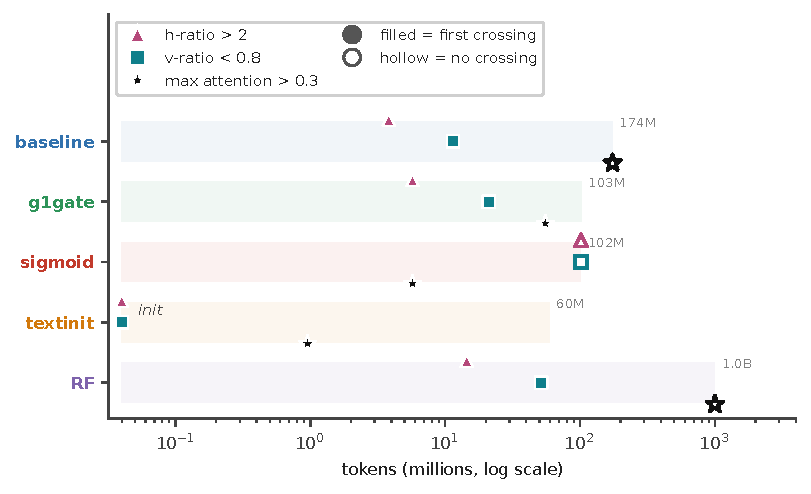
\includegraphics[width=0.8\linewidth]{figures/fig4_leadlag_top.pdf}
  \caption{\textbf{Figure A4: When each signature first crosses threshold.} Seed 0 throughout. Time-to-event tracks spanning the tokens over which we observed each arm (60M to 1B). A filled marker is the first probe at which a signature crossed its threshold (h\&gt;2, v\&lt;0.8, attn$\rightarrow$pos0\&gt;0.3). A hollow marker at a track's end means it never crossed. \textbf{Crossing times are interval-censored} at the 100-step probe cadence (head-level map in Fig. A5).}
  \label{fig:figA4}
\end{figure}

\begin{figure}[t]
  \centering
  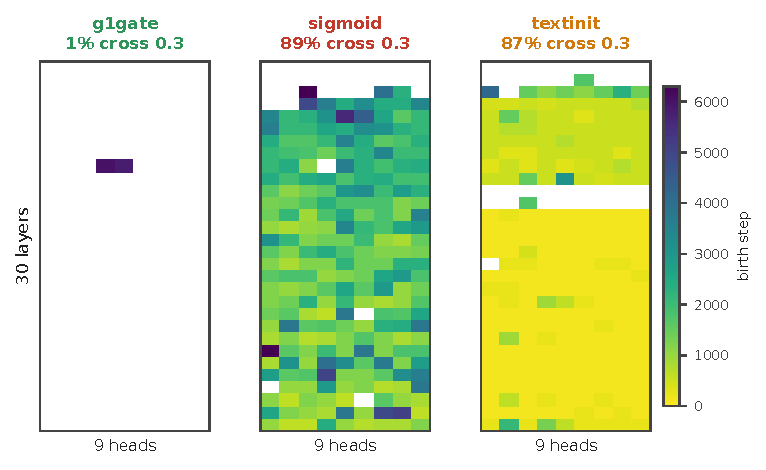
\includegraphics[width=0.8\linewidth]{figures/figA4_birthmap.pdf}
  \caption{\textbf{Figure A5: Birth-maps.} The step at which each (layer, query-head) pair first crosses the concentration threshold (attn\&rarr;pos0 \&gt; 0.3), seed 0, for the three arms in which any head crosses. No \textit{baseline} and no \textit{RF} head ever crosses. 1\% of \textit{g1gate} heads do, against 89\% for \textit{sigmoid} and 87\% for \textit{textinit}. This is the head-level view behind Fig. A4.}
  \label{fig:figA5}
\end{figure}

\paragraph{Timings} In the softmax arms with randomly initialized decoders, \textit{baseline} and \textit{g1gate} and \textit{RF}, the residual-norm ratio crosses its threshold within the first few to about 15M tokens and value-drain follows within about 50M. Concentration never comes. No baseline or RF head ever crosses it, and g1gate reaches 1\% of heads, a single-layer blip late in training. \textit{sigmoid} mirrors that pattern, with concentration crossing at about 6M tokens and 89\% of heads eventually, against 87\% for \textit{textinit}, while neither \textit{sigmoid} norm signature ever crosses (Fig. A5). \textit{textinit} inherits its norm signatures rather than growing them: value-drain and an elevated residual-norm ratio are both present at 0 tokens, imported with the pretrained text-LM weights. Concentration is \textit{not} inherited the same way, since $\mathrm{Sink}^{0.3}_{1}$ is 0.000 at step 0 and crosses before 1M tokens. Even in the arm that imports the most sink structure, the norm signatures precede concentration. Crossing times are interval-censored at the 100-step probe cadence, so two signatures that cross within one interval should not be read as ordered.

\textbf{The sigmoid arm needs one measurement note}, because row-normalization changes the object being measured and Gu et al. \cite{ref6} state their result for \textit{unnormalized} sigmoid attention. The concentration this arm develops is a \textbf{relative} reallocation of a shrinking gate budget onto position 0, not the growth of a large absolute mass there (Appendix D). We report the row-normalized view in the tables so the arms stay comparable.

\paragraph{Entropy collapse} Attention-entropy collapse, the text-LM literature's usual correlate of concentration, separates the same way: only \textit{sigmoid} and \textit{textinit} collapse (Fig. A3). It tracks the concentration axis, not the norm axes.

\paragraph{The signatures also dissociate in position} A per-position scan across all three \textit{textinit} seeds shows they need not share a token. At seed 0 they coincide at position 0. At seed 1 the attention maximum stays there while the residual peak moves to pos1 and the value minimum to pos5. At seed 2 they separate furthest, attention at \textbf{pos1} and both norm extrema at \textbf{pos13}. The arms with randomly initialized decoders behave differently: position 0 stays the maximum-mass token in \textit{baseline}, \textit{g1gate} and \textit{sigmoid} at every seed scanned, and in \textit{RF} the attention argmax sits at pos1 with mass 0.053 against 0.044 at position 0, a diffuse profile rather than a sink (Appendix C).

We report this as a supporting observation, not a second headline. It has one consequence for measurement: because all three metrics anchor on position 0, the \textit{textinit} magnitudes at seeds 1 and 2 are read at a token that is no longer the peak and therefore \textbf{understate} the arm's true peaks, a further reason to report that arm as a range and a median (\S3.1, \S5). The anchoring holds for the randomly initialized decoders, which carry the central negative result.


\newpage
%% NeurIPS Paper Checklist. Mandatory: "The papers not including the checklist will be desk
%% rejected." It follows the references and the appendix, and does not count toward the page
%% limit. Questions and guidelines are reproduced verbatim; only the Answer and Justification
%% lines are ours.
\section*{NeurIPS Paper Checklist}

\begin{enumerate}

\item {\bf Claims}
    \item[] Question: Do the main claims made in the abstract and introduction accurately reflect the paper's contributions and scope?
    \item[] Answer: \answerYes{}
    \item[] Justification: The abstract and Section~1 state exactly the three contributions the paper supports, each with its scope attached: four signature corners at $n = 2$--3 seeds per arm, the low-repetition 1B-token result at a single seed, and the sign-flipping per-head correlation reported at seed 0 and described as descriptive rather than inferential. Section~1 also states plainly that two-way decoupling in text-only models is not ours, and that no downstream behaviour is tested here.
    \item[] Guidelines:
    \begin{itemize}
        \item The answer NA means that the abstract and introduction do not include the claims made in the paper.
        \item The abstract and/or introduction should clearly state the claims made, including the contributions made in the paper and important assumptions and limitations. A No or NA answer to this question will not be perceived well by the reviewers.
        \item The claims made should match theoretical and experimental results, and reflect how much the results can be expected to generalize to other settings.
        \item It is fine to include aspirational goals as motivation as long as it is clear that these goals are not attained by the paper.
    \end{itemize}

\item {\bf Limitations}
    \item[] Question: Does the paper discuss the limitations of the work performed by the authors?
    \item[] Answer: \answerYes{}
    \item[] Justification: Section~5 is a dedicated Limitations section covering position-0 anchoring, the scale confound in the gate arm, the pretrained vision encoder, the h-ratio being a proxy rather than a channel-level measurement of massive activations, token scale, seed-level reproducibility of the textinit magnitudes, provenance and seed counts including the RF optimizer restart, what the RF control cannot establish, domain shift, and the absence of any benchmark accuracy.
    \item[] Guidelines:
    \begin{itemize}
        \item The answer NA means that the paper has no limitation while the answer No means that the paper has limitations, but those are not discussed in the paper.
        \item The authors are encouraged to create a separate "Limitations" section in their paper.
        \item The paper should point out any strong assumptions and how robust the results are to violations of these assumptions.
        \item The authors should reflect on the scope of the claims made, e.g., if the approach was only tested on a few datasets or with a few runs.
        \item The authors should reflect on the factors that influence the performance of the approach.
        \item The authors should discuss the computational efficiency of the proposed algorithms and how they scale with dataset size.
        \item If applicable, the authors should discuss possible limitations of their approach to address problems of privacy and fairness.
        \item While the authors might fear that complete honesty about limitations might be used by reviewers as grounds for rejection, a worse outcome might be that reviewers discover limitations that aren't acknowledged in the paper.
    \end{itemize}

\item {\bf Theory assumptions and proofs}
    \item[] Question: For each theoretical result, does the paper provide the full set of assumptions and a complete (and correct) proof?
    \item[] Answer: \answerNA{}
    \item[] Justification: The paper is empirical and contains no theorems, formal claims or proofs.
    \item[] Guidelines:
    \begin{itemize}
        \item The answer NA means that the paper does not include theoretical results.
        \item All the theorems, formulas, and proofs in the paper should be numbered and cross-referenced.
        \item All assumptions should be clearly stated or referenced in the statement of any theorems.
        \item The proofs can either appear in the main paper or the supplemental material, but if they appear in the supplemental material, the authors are encouraged to provide a short proof sketch to provide intuition.
        \item Inversely, any informal proof provided in the core of the paper should be complemented by formal proofs provided in appendix or supplemental material.
        \item Theorems and Lemmas that the proof relies upon should be properly referenced.
    \end{itemize}

\item {\bf Experimental result reproducibility}
    \item[] Question: Does the paper fully disclose all the information needed to reproduce the main experimental results of the paper to the extent that it affects the main claims and/or conclusions of the paper (regardless of whether the code and data are provided or not)?
    \item[] Answer: \answerYes{}
    \item[] Justification: Section~2 gives the model, token layout, the four training levers, the datasets, the definition of each of the three signatures, the probe and its self-validation tolerance, the optimizer recipe and the seed counts. Appendix~F adds the learning rates, precision, batch size, probe-batch composition, token accounting and the validation protocol. Appendix~B gives the per-seed numbers behind every collapsed range in Table~1.
    \item[] Guidelines:
    \begin{itemize}
        \item The answer NA means that the paper does not include experiments.
        \item If the paper includes experiments, a No answer to this question will not be perceived well by the reviewers: Making the paper reproducible is important, regardless of whether the code and data are provided or not.
        \item If the contribution is a dataset and/or model, the authors should describe the steps taken to make their results reproducible or verifiable.
        \item Depending on the contribution, reproducibility can be accomplished in various ways.
    \end{itemize}

\item {\bf Open access to data and code}
    \item[] Question: Does the paper provide open access to the data and code, with sufficient instructions to faithfully reproduce the main experimental results, as described in supplemental material?
    \item[] Answer: \answerNo{}
    \item[] Justification: The code, probe, run configurations, per-run logs and training checkpoints are prepared for release and the paper commits to releasing them on acceptance, but the links are withheld at submission to preserve double-blind review, and no anonymized mirror is provided. Both datasets used are public and cited. The paper is written so the results can be reproduced from the description alone.
    \item[] Guidelines:
    \begin{itemize}
        \item The answer NA means that paper does not include experiments requiring code.
        \item Please see the NeurIPS code and data submission guidelines for more details.
        \item While we encourage the release of code and data, we understand that this might not be possible, so No is an acceptable answer.
        \item The instructions should contain the exact command and environment needed to run to reproduce the results.
        \item The authors should provide instructions on data access and preparation.
        \item The authors should provide scripts to reproduce all experimental results.
        \item At submission time, to preserve anonymity, the authors should release anonymized versions (if applicable).
    \end{itemize}

\item {\bf Experimental setting/details}
    \item[] Question: Does the paper specify all the training and test details (e.g., data splits, hyperparameters, how they were chosen, type of optimizer) necessary to understand the results?
    \item[] Answer: \answerYes{}
    \item[] Justification: Section~2 specifies the optimizer, weight decay, gradient clipping, schedule and warmup, the token budgets per arm, the held-out split behaviour, and the seed counts. Appendix~F specifies the per-module learning rates, the precision and the batch size. Every arm differs only in the lever under test, which Section~2 states explicitly.
    \item[] Guidelines:
    \begin{itemize}
        \item The answer NA means that the paper does not include experiments.
        \item The experimental setting should be presented in the core of the paper to a level of detail that is necessary to appreciate the results and make sense of them.
        \item The full details can be provided either with the code, in appendix, or as supplemental material.
    \end{itemize}

\item {\bf Experiment statistical significance}
    \item[] Question: Does the paper report error bars suitably and correctly defined or other appropriate information about the statistical significance of the experiments?
    \item[] Answer: \answerNo{}
    \item[] Justification: We report no error bars or significance tests, and say so explicitly. Instead, the main tables give per-arm ranges over 2--3 seeds and Appendix~B gives every per-seed value, so the seed-level variability is fully visible. Section~3.3 states that the per-head correlations are descriptive rather than inferential, because heads within a layer are not independent and each arm rests on a single seed, so a p-value would mislead. Section~5 states that the RF arm is a single seed. With these seed counts, error bars would convey false precision.
    \item[] Guidelines:
    \begin{itemize}
        \item The answer NA means that the paper does not include experiments.
        \item The authors should answer Yes if the results are accompanied by error bars, confidence intervals, or statistical significance tests, at least for the experiments that support the main claims of the paper.
        \item The factors of variability that the error bars are capturing should be clearly stated.
        \item The method for calculating the error bars should be explained.
        \item The assumptions made should be given.
        \item It should be clear whether the error bar is the standard deviation or the standard error of the mean.
        \item It is OK to report 1-sigma error bars, but one should state it.
        \item For asymmetric distributions, the authors should be careful not to show in tables or figures symmetric error bars that would yield results that are out of range.
        \item If error bars are reported in tables or plots, the authors should explain in the text how they were calculated and reference the corresponding figures or tables in the text.
    \end{itemize}

\item {\bf Experiments compute resources}
    \item[] Question: For each experiment, does the paper provide sufficient information on the computer resources (type of compute workers, memory, time of execution) needed to reproduce the experiments?
    \item[] Answer: \answerNo{}
    \item[] Justification: The paper states the token budget of every run, which fixes the dominant cost, but it does not state the accelerator type, memory or wall-clock time. Two memory-driven events are disclosed in Section~5, the weights-only optimizer restart in the RF run and the reduction of the streaming shuffle buffer, because they affect interpretation of the results rather than only the cost.
    \item[] Guidelines:
    \begin{itemize}
        \item The answer NA means that the paper does not include experiments.
        \item The paper should indicate the type of compute workers CPU or GPU, internal cluster, or cloud provider, including relevant memory and storage.
        \item The paper should provide the amount of compute required for each of the individual experimental runs as well as estimate the total compute.
        \item The paper should disclose whether the full research project required more compute than the experiments reported in the paper.
    \end{itemize}

\item {\bf Code of ethics}
    \item[] Question: Does the research conducted in the paper conform, in every respect, with the NeurIPS Code of Ethics?
    \item[] Answer: \answerYes{}
    \item[] Justification: The work trains small vision--language models on public, already-published image--text corpora, involves no human subjects and no personal data, and releases no model with foreseeable misuse potential. Anonymity is preserved in this submission.
    \item[] Guidelines:
    \begin{itemize}
        \item The answer NA means that the authors have not reviewed the NeurIPS Code of Ethics.
        \item If the authors answer No, they should explain the special circumstances that require a deviation from the Code of Ethics.
        \item The authors should make sure to preserve anonymity.
    \end{itemize}

\item {\bf Broader impacts}
    \item[] Question: Does the paper discuss both potential positive societal impacts and negative societal impacts of the work performed?
    \item[] Answer: \answerNA{}
    \item[] Justification: This is foundational measurement work on the internal mechanics of 222M-parameter research models. It proposes no application, releases no deployable system, and improves no capability. Its practical consequence is confined to how interpretability and mitigation work reports attention sinks, which the Conclusion states.
    \item[] Guidelines:
    \begin{itemize}
        \item The answer NA means that there is no societal impact of the work performed.
        \item If the authors answer NA or No, they should explain why their work has no societal impact or why the paper does not address societal impact.
        \item Examples of negative societal impacts include potential malicious or unintended uses, fairness considerations, privacy considerations, and security considerations.
        \item The conference expects that many papers will be foundational research and not tied to particular applications, let alone deployments.
        \item The authors should consider possible harms that could arise when the technology is being used as intended and functioning correctly, harms that could arise when the technology is being used as intended but gives incorrect results, and harms following from misuse of the technology.
        \item If there are negative societal impacts, the authors could also discuss possible mitigation strategies.
    \end{itemize}

\item {\bf Safeguards}
    \item[] Question: Does the paper describe safeguards that have been put in place for responsible release of data or models that have a high risk for misuse (e.g., pre-trained language models, image generators, or scraped datasets)?
    \item[] Answer: \answerNA{}
    \item[] Justification: The artefacts are 222M-parameter research checkpoints trained for a measurement study. They are far below any capability threshold that would carry misuse risk, and no dataset is released.
    \item[] Guidelines:
    \begin{itemize}
        \item The answer NA means that the paper poses no such risks.
        \item Released models that have a high risk for misuse or dual-use should be released with necessary safeguards to allow for controlled use of the model.
        \item Datasets that have been scraped from the Internet could pose safety risks. The authors should describe how they avoided releasing unsafe images.
        \item We recognize that providing effective safeguards is challenging, and many papers do not require this, but we encourage authors to take this into account and make a best faith effort.
    \end{itemize}

\item {\bf Licenses for existing assets}
    \item[] Question: Are the creators or original owners of assets (e.g., code, data, models), used in the paper, properly credited and are the license and terms of use explicitly mentioned and properly respected?
    \item[] Answer: \answerNo{}
    \item[] Justification: Every existing asset is cited to its original paper at the point of use: the nanoVLM codebase, the SigLIP-B/16 encoder, the SmolLM2 architecture and weights, and both image--text corpora. The paper does not, however, enumerate the license of each asset by name, so this answer is No rather than Yes. All assets are publicly released for research use and were used within those terms.
    \item[] Guidelines:
    \begin{itemize}
        \item The answer NA means that the paper does not use existing assets.
        \item The authors should cite the original paper that produced the code package or dataset.
        \item The authors should state which version of the asset is used and, if possible, include a URL.
        \item The name of the license (e.g., CC-BY 4.0) should be included for each asset.
        \item For scraped data from a particular source, the copyright and terms of service of that source should be provided.
        \item If assets are released, the license, copyright information, and terms of use in the package should be provided.
        \item For existing datasets that are re-packaged, both the original license and the license of the derived asset should be provided.
        \item If this information is not available online, the authors are encouraged to reach out to the asset's creators.
    \end{itemize}

\item {\bf New assets}
    \item[] Question: Are new assets introduced in the paper well documented and is the documentation provided alongside the assets?
    \item[] Answer: \answerNA{}
    \item[] Justification: No new asset is released with this submission. The code, probe, run configurations, logs and checkpoints are held for release on acceptance, at which point they will carry documentation.
    \item[] Guidelines:
    \begin{itemize}
        \item The answer NA means that the paper does not release new assets.
        \item Researchers should communicate the details of the dataset/code/model as part of their submissions via structured templates.
        \item The paper should discuss whether and how consent was obtained from people whose asset is used.
        \item At submission time, remember to anonymize your assets (if applicable).
    \end{itemize}

\item {\bf Crowdsourcing and research with human subjects}
    \item[] Question: For crowdsourcing experiments and research with human subjects, does the paper include the full text of instructions given to participants and screenshots, if applicable, as well as details about compensation (if any)?
    \item[] Answer: \answerNA{}
    \item[] Justification: The work involves no crowdsourcing and no human subjects.
    \item[] Guidelines:
    \begin{itemize}
        \item The answer NA means that the paper does not involve crowdsourcing nor research with human subjects.
        \item Including this information in the supplemental material is fine, but if the main contribution of the paper involves human subjects, then as much detail as possible should be included in the main paper.
        \item According to the NeurIPS Code of Ethics, workers involved in data collection, curation, or other labor should be paid at least the minimum wage in the country of the data collector.
    \end{itemize}

\item {\bf Institutional review board (IRB) approvals or equivalent for research with human subjects}
    \item[] Question: Does the paper describe potential risks incurred by study participants, whether such risks were disclosed to the subjects, and whether Institutional Review Board (IRB) approvals (or an equivalent approval/review based on the requirements of your country or institution) were obtained?
    \item[] Answer: \answerNA{}
    \item[] Justification: The work involves no human subjects, so no IRB review or equivalent applies.
    \item[] Guidelines:
    \begin{itemize}
        \item The answer NA means that the paper does not involve crowdsourcing nor research with human subjects.
        \item Depending on the country in which research is conducted, IRB approval (or equivalent) may be required for any human subjects research.
        \item We recognize that the procedures for this may vary significantly between institutions and locations, and we expect authors to adhere to the NeurIPS Code of Ethics and the guidelines for their institution.
        \item For initial submissions, do not include any information that would break anonymity.
    \end{itemize}

\item {\bf Declaration of LLM usage}
    \item[] Question: Does the paper describe the usage of LLMs if it is an important, original, or non-standard component of the core methods in this research? Note that if the LLM is used only for writing, editing, or formatting purposes and does not impact the core methodology, scientific rigor, or originality of the research, declaration is not required.
    \item[] Answer: \answerNA{}
    \item[] Justification: Language models appear in this work only as the object of study, a 135M-parameter decoder trained and probed by the authors. No large language model forms part of the method, and any use in writing or editing does not affect the methodology, results or originality.
    \item[] Guidelines:
    \begin{itemize}
        \item The answer NA means that the core method development in this research does not involve LLMs as any important, original, or non-standard components.
        \item Please refer to our LLM policy in the NeurIPS handbook for what should or should not be described.
    \end{itemize}

\end{enumerate}



\end{document}
